\begin{frame}[parent={ie:agenda}, hasnext=true, hasprev=false]
	\frametitle{Dromey}

	\begin{block:concept}{Modelo de Dromey}
		Qualidade definida pela avaliação de propriedades de qualidade quanto às
		características do produto
		\begin{itemize}
			\item Produto organizado em componentes (\foreign{structural form})
			
			\item Avaliação a partir de violação das propriedades de qualidade
			(\foreign{quality defect})
		\end{itemize}
	
		Qualidade é evitar os defeitos de qualidade!
	\end{block:concept}
	
	\begin{block:fact}{}
		\centering
		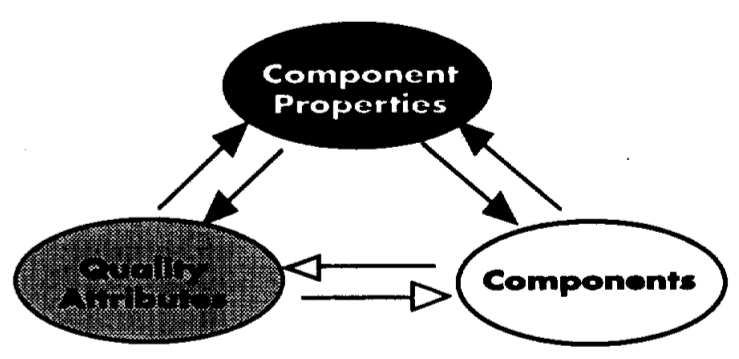
\includegraphics[width=.6\textwidth]{software-engineering/project-management/product/dromey/dromey-generic_model}
	\end{block:fact}
\end{frame}



\begin{frame}[hasnext=true, hasprev=true]
	\frametitle{Dromey}
	\framesubtitle{Structural form}

	\begin{block:fact}{Structural form}
		\begin{itemize}
			\item Estabelecido pela sintaxe da linguagem (no caso do estudo, linguagem
			de programação)
		\end{itemize}
	\end{block:fact}
	
	\begin{block:fact}{Structural forms: processos e dados}
		\centering
		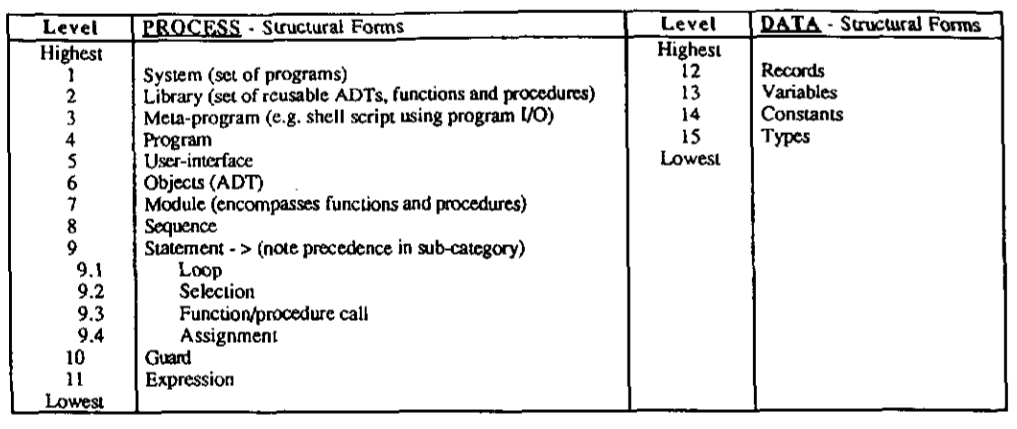
\includegraphics[width=\textwidth]{software-engineering/project-management/product/dromey/dromey-structural_forms}
	\end{block:fact}
\end{frame}



\begin{frame}
	\frametitle{Dromey}
	\framesubtitle{Atributos de qualidade}
	
	\begin{block:fact}{Atributos de qualidade}
		\begin{itemize}
			\item Funcionalidade
			\item Confiabilidade
			\item Usabilidade
			\item Eficiência
			\item Manutenibilidade
			\item Portabilidade
			\item \textbf{Reusabilidade}
		\end{itemize}
	\end{block:fact}
	
	\note{
		Os seis primeiros advém da ISO 9126.
	}
\end{frame}


\begin{frame}
	\frametitle{Dromey}
	\framesubtitle{Propriedades de qualidade}
	
	\begin{block:fact}{Atributos de qualidade e suas propriedades}
		\begin{itemize}
			\item Cada atributo está relacionado com uma ou mais propriedades de qualidade.
			
			\item Tipos de propriedades (em prioridade):
			\begin{itemize}
				\item Correção
				\item Estrutura
				\item Modularidade
				\item Descriptividade/Descrição
			\end{itemize}
		\end{itemize}
	\end{block:fact}

	\note{
		Critério para a definição das propriedades dentro de cada categoria:
		\begin{itemize}
			\item ortogonalidade,
			\item consistência,
			\item completude.
		\end{itemize}
	}
\end{frame}


\begin{frame}
	\frametitle{Dromey}
	\framesubtitle{Exemplo}

	\begin{block:fact}{Propriedade: Correctness (C1: Computable)}
		\centering
		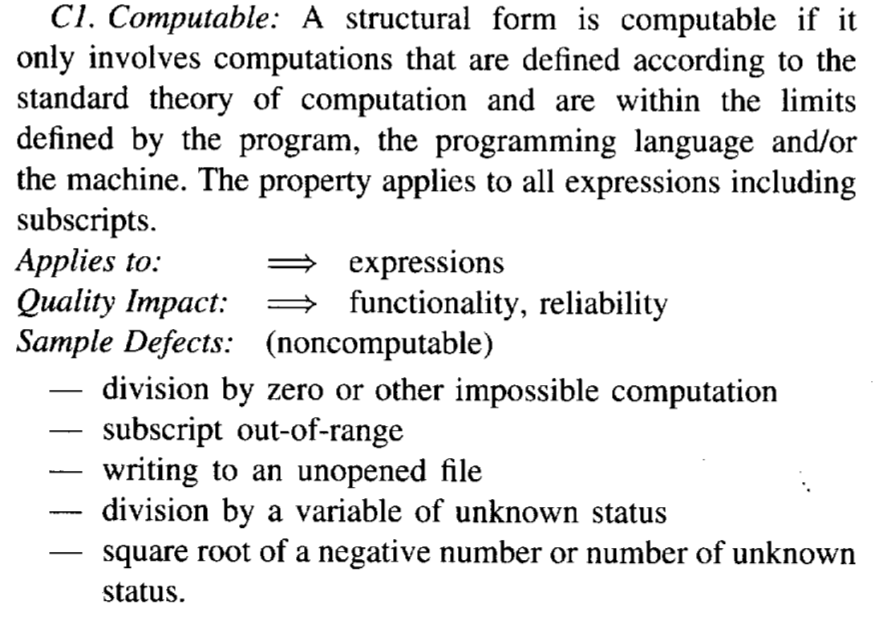
\includegraphics[width=.7\textwidth]{software-engineering/project-management/product/dromey/dromey-property_example}
	\end{block:fact}

\end{frame}



\begin{frame}
	\frametitle{Dromey}
	\framesubtitle{Propriedades de qualidade}
	
	\begin{block:fact}{Structural forms e propriedades dos atributos de qualidade}
		\begin{itemize}
			\item Cada \foreign{structural form} está relacionado com uma ou mais
			propriedades de qualidade
		\end{itemize}
	\end{block:fact}
\end{frame}


\begin{frame}
	\frametitle{Dromey}
	\framesubtitle{Propriedades de qualidade}
	
	\begin{block:fact}{Structural forms e propriedades dos atributos de qualidade}
		\centering
		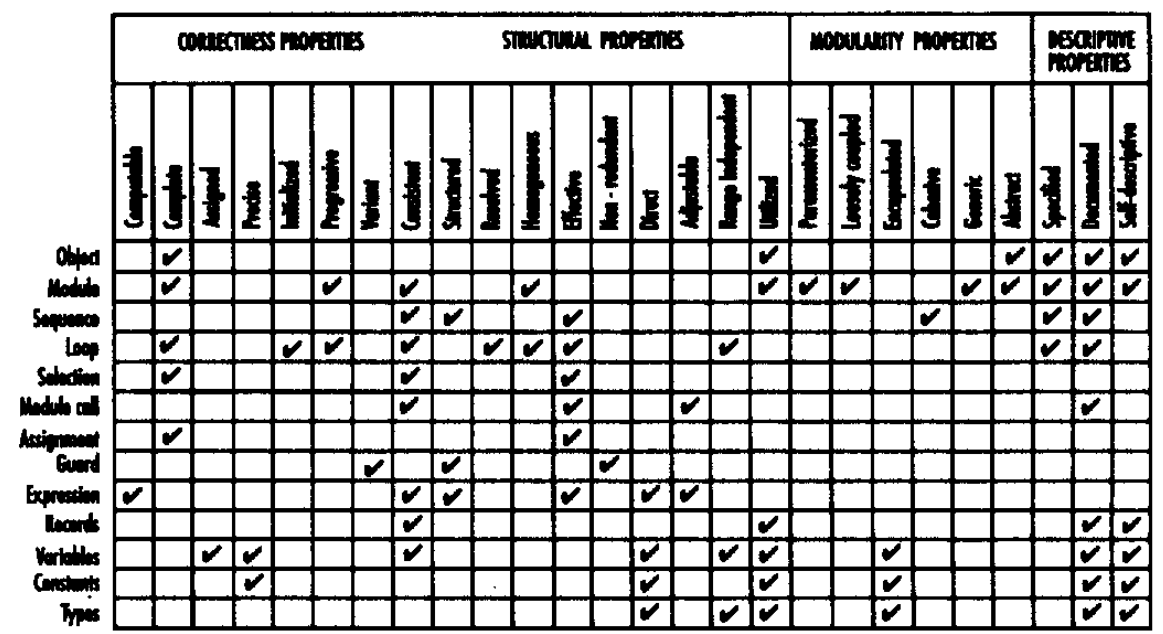
\includegraphics[width=\textwidth]{software-engineering/project-management/product/dromey/dromey-structural_forms_X_properties}
	\end{block:fact}
\end{frame}


\begin{frame}
	\frametitle{Dromey}
	\framesubtitle{Propriedades de qualidade}
	
 	\begin{block:fact}{Propriedades dos atributos de qualidade e fatores de qualidade}
		\centering
		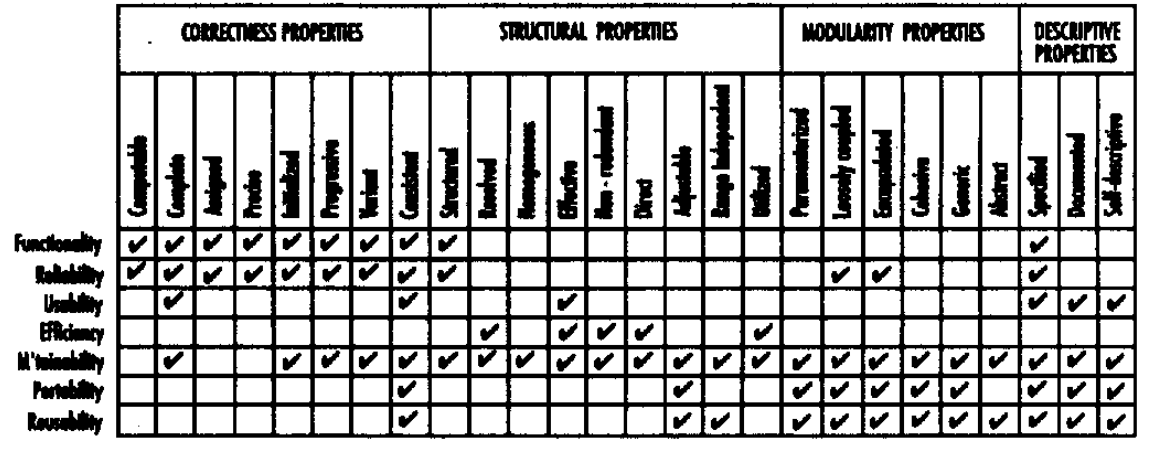
\includegraphics[width=\textwidth]{software-engineering/project-management/product/dromey/dromey-properties_X_quality}
	\end{block:fact}
\end{frame}



\begin{frame}
	\frametitle{Dromey}
	
	\begin{block:fact}{Considerações finais}
		\begin{itemize}
			\item Passível de automatização
			
			\item Não é apenas um modelo, mas um método para definir um modelo
			\begin{itemize}
				\item Identifica defeitos de qualidade, defina uma nova propriedade
				relacionada a um \foreign{structural form}
			\end{itemize}
			
			\item Não avalia diretamente a qualidade em uso
		\end{itemize}
	\end{block:fact}
\end{frame}

